\SourceLeaf{197}\clearpage
\begin{center}
[ÜBER DIE WINKEL DES DREIECKS.]
\end{center}

\begin{center}
[1.]
\end{center}

Der Beweis, dass die Summe der drei Winkel eines Dreiecks nicht grösser sein
kann als $180^{0}$, ist unabhängig vom 11. Axiom so zu führen.



\begin{center}
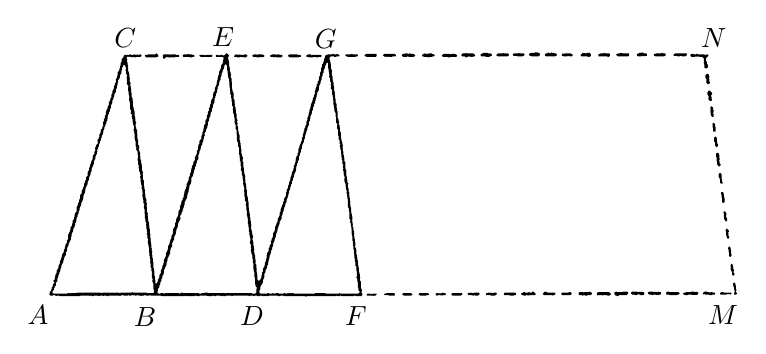
\begin{tikzpicture}[x=0.00629183cm,y=-0.00629183cm]
\fill[even odd rule] (706,574) -- (707,575) -- (718,575) -- (720,576) -- (721,575) -- (724,575) -- (726,573) -- (726,572) -- (725,571) -- (723,571) -- (722,572) -- (720,571) -- (718,572) -- (708,571) -- (706,573) -- cycle
(877,572) -- (877,573) -- (879,575) -- (896,575) -- (899,573) -- (899,571) -- (898,570) -- (879,570) -- cycle
(811,572) -- (811,573) -- (814,575) -- (826,575) -- (827,574) -- (831,574) -- (832,573) -- (832,572) -- (829,570) -- (813,570) -- cycle
(778,572) -- (778,573) -- (781,575) -- (796,575) -- (798,573) -- (798,572) -- (795,570) -- (780,570) -- cycle
(741,572) -- (742,574) -- (750,574) -- (751,575) -- (762,575) -- (763,574) -- (763,572) -- (761,570) -- (746,570) -- (745,571) -- (742,571) -- cycle
(983,571) -- (983,573) -- (984,574) -- (994,574) -- (995,575) -- (1003,575) -- (1004,574) -- (1007,574) -- (1008,573) -- (1008,571) -- (1006,569) -- (985,569) -- cycle
(947,571) -- (947,573) -- (948,574) -- (956,574) -- (957,575) -- (965,575) -- (969,572) -- (969,571) -- (967,569) -- (964,569) -- (963,570) -- (952,569) -- (951,570) -- (948,570) -- cycle
(910,571) -- (910,572) -- (912,574) -- (919,574) -- (920,575) -- (922,575) -- (923,574) -- (925,575) -- (931,575) -- (934,572) -- (934,571) -- (932,569) -- (923,569) -- (922,570) -- (918,570) -- (917,569) -- (915,569) -- (914,570) -- (911,570) -- cycle
(866,572) -- (864,570) -- (861,570) -- (859,569) -- (856,571) -- (847,570) -- (845,572) -- (845,573) -- (847,575) -- (849,575) -- (850,574) -- (860,575) -- (861,574) -- (865,574) -- cycle
(1420,570) -- (1420,572) -- (1421,573) -- (1433,573) -- (1434,572) -- (1439,572) -- (1441,573) -- (1443,571) -- (1442,569) -- (1427,569) -- (1426,568) -- (1423,568) -- cycle
(1171,570) -- (1171,573) -- (1173,575) -- (1175,574) -- (1181,574) -- (1182,575) -- (1184,574) -- (1191,574) -- (1192,575) -- (1196,575) -- (1199,573) -- (1199,571) -- (1195,568) -- (1174,568) -- cycle
(1120,570) -- (1117,568) -- (1115,568) -- (1114,569) -- (1101,569) -- (1099,571) -- (1099,572) -- (1101,574) -- (1118,574) -- (1120,572) -- cycle
(1385,570) -- (1385,572) -- (1386,573) -- (1389,572) -- (1390,573) -- (1398,573) -- (1399,574) -- (1403,574) -- (1404,573) -- (1409,573) -- (1410,572) -- (1410,570) -- (1409,569) -- (1405,569) -- (1404,568) -- (1398,569) -- (1397,568) -- (1394,568) -- (1393,567) -- (1389,567) -- cycle
(1376,570) -- (1374,568) -- (1362,567) -- (1361,568) -- (1351,568) -- (1350,569) -- (1347,569) -- (1345,571) -- (1345,572) -- (1349,574) -- (1354,574) -- (1355,573) -- (1372,574) -- (1374,573) -- (1376,571) -- cycle
(1311,569) -- (1311,572) -- (1312,573) -- (1317,573) -- (1318,574) -- (1333,574) -- (1334,573) -- (1336,573) -- (1338,571) -- (1338,570) -- (1335,568) -- (1317,568) -- (1316,567) -- (1314,567) -- cycle
(1274,569) -- (1274,571) -- (1277,573) -- (1281,573) -- (1282,574) -- (1284,574) -- (1285,573) -- (1296,574) -- (1297,573) -- (1299,573) -- (1301,571) -- (1301,569) -- (1300,568) -- (1297,568) -- (1296,567) -- (1294,568) -- (1277,567) -- cycle
(1240,569) -- (1240,571) -- (1242,573) -- (1247,573) -- (1248,574) -- (1251,574) -- (1255,572) -- (1259,574) -- (1265,574) -- (1267,572) -- (1267,570) -- (1265,568) -- (1243,567) -- cycle
(1206,569) -- (1207,573) -- (1209,575) -- (1211,575) -- (1212,576) -- (1214,576) -- (1216,574) -- (1231,574) -- (1234,571) -- (1234,569) -- (1232,567) -- (1224,567) -- (1223,568) -- (1212,568) -- (1210,567) -- cycle
(1161,571) -- (1159,568) -- (1157,568) -- (1156,567) -- (1154,568) -- (1145,568) -- (1144,569) -- (1142,568) -- (1136,568) -- (1134,570) -- (1134,573) -- (1135,574) -- (1140,574) -- (1141,575) -- (1143,575) -- (1144,574) -- (1146,574) -- (1147,575) -- (1151,575) -- (1152,574) -- (1159,574) -- (1161,572) -- cycle
(1062,571) -- (1062,572) -- (1064,574) -- (1080,574) -- (1081,575) -- (1085,574) -- (1087,572) -- (1087,570) -- (1086,569) -- (1071,569) -- (1068,567) -- (1065,568) -- cycle
(1047,573) -- (1047,571) -- (1043,567) -- (1041,567) -- (1039,569) -- (1035,569) -- (1034,568) -- (1032,569) -- (1026,569) -- (1025,568) -- (1023,568) -- (1021,570) -- (1019,570) -- (1018,571) -- (1018,572) -- (1020,574) -- (1022,574) -- (1023,575) -- (1027,575) -- (1028,574) -- (1034,575) -- (1035,574) -- (1046,574) -- cycle
(1448,549) -- (1446,551) -- (1447,557) -- (1448,558) -- (1448,563) -- (1449,564) -- (1449,569) -- (1448,570) -- (1448,572) -- (1449,573) -- (1452,573) -- (1454,571) -- (1454,570) -- (1452,568) -- (1452,566) -- (1453,565) -- (1453,563) -- (1452,562) -- (1452,555) -- (1451,554) -- (1451,551) -- (1449,549) -- cycle
(1443,511) -- (1441,513) -- (1441,517) -- (1442,518) -- (1441,522) -- (1444,528) -- (1444,533) -- (1446,535) -- (1447,535) -- (1449,532) -- (1449,531) -- (1447,529) -- (1447,526) -- (1448,524) -- (1446,520) -- (1446,515) -- (1445,514) -- (1445,512) -- cycle
(1438,476) -- (1436,479) -- (1436,481) -- (1437,482) -- (1437,487) -- (1438,488) -- (1438,495) -- (1440,497) -- (1441,497) -- (1443,494) -- (1443,492) -- (1442,491) -- (1442,483) -- (1441,482) -- (1441,479) -- (1440,477) -- cycle
(1433,440) -- (1431,443) -- (1431,445) -- (1432,446) -- (1432,453) -- (1433,454) -- (1433,457) -- (1435,460) -- (1437,460) -- (1438,459) -- (1438,455) -- (1436,453) -- (1437,451) -- (1436,448) -- (1438,446) -- (1437,443) -- (1434,440) -- cycle
(1428,405) -- (1427,406) -- (1428,420) -- (1431,425) -- (1433,425) -- (1434,424) -- (1434,419) -- (1432,417) -- (1432,412) -- (1433,410) -- (1430,405) -- cycle
(1423,366) -- (1422,367) -- (1422,371) -- (1423,372) -- (1423,377) -- (1424,378) -- (1424,386) -- (1426,388) -- (1427,388) -- (1429,386) -- (1429,378) -- (1428,377) -- (1427,368) -- (1425,366) -- cycle
(1419,327) -- (1417,331) -- (1417,335) -- (1420,341) -- (1420,347) -- (1422,349) -- (1424,349) -- (1425,348) -- (1425,346) -- (1424,345) -- (1424,341) -- (1423,340) -- (1423,331) -- (1422,329) -- (1420,327) -- cycle
(1413,287) -- (1412,288) -- (1412,295) -- (1413,296) -- (1413,304) -- (1414,305) -- (1414,310) -- (1417,314) -- (1419,314) -- (1421,312) -- (1421,310) -- (1419,308) -- (1419,305) -- (1418,304) -- (1418,302) -- (1419,301) -- (1418,289) -- (1416,287) -- cycle
(1410,254) -- (1408,256) -- (1408,264) -- (1410,266) -- (1410,272) -- (1412,275) -- (1414,275) -- (1416,271) -- (1414,267) -- (1413,256) -- (1411,254) -- cycle
(1406,226) -- (1405,227) -- (1405,236) -- (1406,237) -- (1406,243) -- (1407,244) -- (1410,244) -- (1411,243) -- (1411,235) -- (1410,234) -- (1410,229) -- (1407,226) -- cycle
(1402,193) -- (1400,195) -- (1400,198) -- (1401,199) -- (1401,201) -- (1400,202) -- (1401,204) -- (1401,209) -- (1402,210) -- (1402,212) -- (1404,214) -- (1406,214) -- (1407,213) -- (1407,209) -- (1406,208) -- (1407,201) -- (1406,200) -- (1406,197) -- (1405,195) -- (1403,193) -- cycle
(1397,161) -- (1394,165) -- (1394,168) -- (1397,173) -- (1396,178) -- (1399,182) -- (1402,182) -- (1404,180) -- (1403,178) -- (1403,174) -- (1402,173) -- (1402,170) -- (1404,168) -- (1404,166) -- (1399,161) -- cycle
(1393,127) -- (1390,130) -- (1390,135) -- (1392,137) -- (1392,145) -- (1395,148) -- (1397,148) -- (1399,146) -- (1399,144) -- (1398,143) -- (1398,138) -- (1397,137) -- (1398,135) -- (1398,132) -- (1397,131) -- (1397,129) -- (1395,127) -- cycle
(368,90) -- (368,91) -- (371,93) -- (393,93) -- (394,92) -- (394,90) -- (393,89) -- (381,89) -- (380,90) -- (378,89) -- (369,89) -- cycle
(584,90) -- (584,92) -- (585,93) -- (588,93) -- (589,94) -- (597,94) -- (598,93) -- (607,94) -- (608,93) -- (613,93) -- (615,91) -- (614,89) -- (597,89) -- (595,90) -- (593,88) -- (588,88) -- cycle
(547,90) -- (547,91) -- (550,94) -- (568,94) -- (569,93) -- (572,93) -- (573,92) -- (573,90) -- (572,89) -- (567,89) -- (566,88) -- (550,88) -- cycle
(511,90) -- (511,92) -- (512,93) -- (517,93) -- (518,94) -- (520,93) -- (522,93) -- (523,94) -- (533,94) -- (536,91) -- (535,89) -- (530,89) -- (529,88) -- (525,88) -- (524,89) -- (522,88) -- (515,88) -- cycle
(475,90) -- (475,91) -- (477,93) -- (483,93) -- (484,94) -- (498,93) -- (499,92) -- (499,90) -- (495,88) -- (486,88) -- (485,89) -- (483,88) -- (478,88) -- cycle
(438,92) -- (439,93) -- (443,93) -- (444,94) -- (449,94) -- (450,93) -- (462,94) -- (465,91) -- (465,90) -- (463,88) -- (459,88) -- (458,89) -- (441,88) -- (438,91) -- cycle
(294,90) -- (294,93) -- (296,97) -- (297,97) -- (301,93) -- (303,93) -- (304,94) -- (318,94) -- (319,93) -- (326,93) -- (327,92) -- (327,90) -- (326,89) -- (321,89) -- (320,88) -- (310,88) -- (309,89) -- (307,88) -- (296,88) -- cycle
(1360,89) -- (1360,91) -- (1362,93) -- (1369,93) -- (1370,92) -- (1384,93) -- (1387,96) -- (1387,107) -- (1388,108) -- (1388,114) -- (1390,116) -- (1393,116) -- (1395,114) -- (1395,109) -- (1393,106) -- (1393,103) -- (1391,100) -- (1391,96) -- (1396,91) -- (1396,89) -- (1395,88) -- (1389,89) -- (1388,88) -- (1375,88) -- (1374,87) -- (1372,87) -- (1371,88) -- (1367,88) -- (1366,87) -- (1362,87) -- cycle
(858,90) -- (858,91) -- (860,93) -- (870,93) -- (871,94) -- (874,94) -- (875,93) -- (887,93) -- (888,92) -- (888,89) -- (884,87) -- (876,87) -- (875,88) -- (873,87) -- (861,87) -- cycle
(739,89) -- (739,90) -- (743,93) -- (745,92) -- (747,93) -- (749,93) -- (750,92) -- (752,93) -- (757,93) -- (758,92) -- (764,92) -- (765,91) -- (765,89) -- (763,87) -- (742,87) -- cycle
(702,89) -- (702,91) -- (706,93) -- (724,93) -- (726,91) -- (726,88) -- (725,87) -- (705,87) -- cycle
(663,89) -- (663,90) -- (665,92) -- (667,92) -- (668,93) -- (683,93) -- (684,92) -- (687,92) -- (688,91) -- (688,89) -- (687,88) -- (678,88) -- (677,87) -- (675,87) -- (674,88) -- (664,88) -- cycle
(334,90) -- (334,91) -- (336,93) -- (348,93) -- (349,94) -- (353,94) -- (354,93) -- (357,93) -- (358,92) -- (358,90) -- (357,89) -- (354,89) -- (353,88) -- (347,88) -- (346,87) -- (344,88) -- (336,88) -- cycle
(1326,88) -- (1326,90) -- (1327,91) -- (1333,91) -- (1334,92) -- (1338,92) -- (1339,91) -- (1342,91) -- (1343,92) -- (1349,92) -- (1353,89) -- (1353,87) -- (1352,86) -- (1329,86) -- cycle
(1100,88) -- (1100,90) -- (1104,92) -- (1111,92) -- (1112,91) -- (1120,92) -- (1122,90) -- (1122,88) -- (1118,86) -- (1106,86) -- (1105,87) -- (1102,86) -- cycle
(818,89) -- (818,91) -- (819,92) -- (821,92) -- (822,93) -- (829,93) -- (830,94) -- (832,94) -- (833,93) -- (838,93) -- (839,92) -- (842,92) -- (843,91) -- (843,89) -- (842,88) -- (838,87) -- (837,86) -- (831,86) -- (830,87) -- (822,86) -- cycle
(777,89) -- (777,91) -- (781,93) -- (787,93) -- (788,92) -- (790,92) -- (791,93) -- (800,93) -- (804,91) -- (804,90) -- (802,88) -- (800,87) -- (795,87) -- (794,86) -- (792,86) -- (791,87) -- (789,87) -- (788,86) -- (783,86) -- (782,87) -- (779,87) -- cycle
(651,90) -- (649,88) -- (647,88) -- (646,87) -- (644,88) -- (640,88) -- (639,87) -- (637,87) -- (636,88) -- (627,88) -- (626,89) -- (624,89) -- (622,91) -- (622,94) -- (620,97) -- (620,100) -- (619,101) -- (618,106) -- (616,108) -- (616,112) -- (614,116) -- (614,121) -- (612,125) -- (612,130) -- (610,133) -- (609,141) -- (607,143) -- (607,147) -- (605,149) -- (605,152) -- (603,156) -- (603,159) -- (601,162) -- (601,168) -- (599,171) -- (599,174) -- (597,177) -- (597,180) -- (596,181) -- (596,183) -- (593,190) -- (593,193) -- (592,194) -- (592,197) -- (590,201) -- (590,205) -- (589,206) -- (588,213) -- (586,216) -- (586,221) -- (584,224) -- (584,230) -- (582,232) -- (582,235) -- (580,238) -- (580,241) -- (579,242) -- (578,248) -- (577,249) -- (577,254) -- (575,257) -- (575,263) -- (573,265) -- (573,267) -- (570,273) -- (570,276) -- (568,279) -- (568,286) -- (566,288) -- (567,291) -- (564,294) -- (564,296) -- (563,297) -- (562,306) -- (561,307) -- (561,310) -- (559,312) -- (559,317) -- (558,318) -- (558,321) -- (557,322) -- (557,324) -- (555,326) -- (555,330) -- (554,331) -- (554,333) -- (552,337) -- (552,340) -- (549,347) -- (549,350) -- (547,354) -- (547,357) -- (544,363) -- (544,366) -- (543,367) -- (543,373) -- (539,380) -- (539,383) -- (537,387) -- (537,390) -- (535,392) -- (535,394) -- (532,401) -- (532,405) -- (530,408) -- (530,413) -- (526,421) -- (526,426) -- (524,428) -- (524,430) -- (521,437) -- (521,442) -- (520,443) -- (520,445) -- (517,449) -- (517,455) -- (516,456) -- (516,458) -- (514,460) -- (514,463) -- (512,467) -- (513,470) -- (510,474) -- (510,477) -- (508,480) -- (508,485) -- (505,489) -- (505,492) -- (504,493) -- (504,500) -- (503,501) -- (503,504) -- (500,510) -- (500,514) -- (499,515) -- (499,517) -- (497,520) -- (496,527) -- (495,528) -- (494,534) -- (493,535) -- (493,539) -- (491,543) -- (489,545) -- (487,545) -- (485,542) -- (485,533) -- (484,532) -- (483,513) -- (481,510) -- (482,505) -- (481,504) -- (481,500) -- (480,499) -- (481,495) -- (480,494) -- (479,488) -- (478,487) -- (479,481) -- (478,480) -- (478,475) -- (477,474) -- (477,467) -- (476,466) -- (476,463) -- (475,462) -- (475,460) -- (476,459) -- (476,454) -- (475,453) -- (474,444) -- (473,443) -- (473,440) -- (472,439) -- (473,432) -- (472,431) -- (472,425) -- (471,424) -- (471,418) -- (470,417) -- (470,410) -- (469,409) -- (469,405) -- (468,404) -- (467,384) -- (466,383) -- (466,377) -- (465,376) -- (465,373) -- (464,372) -- (464,362) -- (463,361) -- (462,349) -- (461,348) -- (460,331) -- (458,328) -- (459,325) -- (458,324) -- (458,317) -- (457,316) -- (457,311) -- (456,310) -- (457,306) -- (455,303) -- (456,296) -- (454,293) -- (454,290) -- (453,289) -- (453,280) -- (452,279) -- (451,267) -- (450,266) -- (450,262) -- (449,261) -- (449,251) -- (448,250) -- (448,248) -- (447,247) -- (447,243) -- (446,242) -- (446,234) -- (444,231) -- (445,229) -- (445,227) -- (444,226) -- (444,223) -- (445,221) -- (443,217) -- (443,208) -- (442,207) -- (441,195) -- (439,192) -- (440,188) -- (439,187) -- (439,180) -- (437,178) -- (437,166) -- (435,163) -- (435,160) -- (434,159) -- (433,137) -- (431,133) -- (432,128) -- (431,127) -- (431,124) -- (429,121) -- (430,117) -- (429,116) -- (429,113) -- (428,112) -- (428,102) -- (427,101) -- (427,98) -- (426,97) -- (426,93) -- (428,91) -- (428,90) -- (424,86) -- (422,86) -- (418,90) -- (415,90) -- (414,89) -- (410,89) -- (409,90) -- (407,90) -- (406,89) -- (402,89) -- (401,90) -- (401,92) -- (402,93) -- (415,93) -- (417,95) -- (415,106) -- (412,110) -- (412,115) -- (408,123) -- (408,128) -- (406,131) -- (406,134) -- (405,135) -- (405,140) -- (404,141) -- (404,144) -- (403,145) -- (403,149) -- (401,151) -- (401,153) -- (399,156) -- (399,162) -- (396,165) -- (396,168) -- (395,169) -- (396,173) -- (395,174) -- (394,178) -- (392,180) -- (391,187) -- (389,191) -- (390,194) -- (387,197) -- (388,201) -- (385,204) -- (385,209) -- (383,212) -- (383,217) -- (380,222) -- (380,228) -- (377,232) -- (377,237) -- (376,238) -- (376,242) -- (374,246) -- (374,249) -- (372,253) -- (372,258) -- (368,263) -- (368,268) -- (366,271) -- (365,280) -- (363,283) -- (363,288) -- (359,296) -- (359,301) -- (356,305) -- (356,309) -- (353,314) -- (353,317) -- (352,318) -- (351,325) -- (349,329) -- (349,332) -- (346,338) -- (346,343) -- (344,345) -- (344,347) -- (342,350) -- (342,355) -- (341,356) -- (341,359) -- (339,361) -- (339,363) -- (338,364) -- (337,372) -- (336,373) -- (336,377) -- (334,379) -- (334,382) -- (332,384) -- (331,391) -- (329,394) -- (329,400) -- (326,404) -- (325,414) -- (322,418) -- (322,420) -- (321,421) -- (321,425) -- (319,429) -- (319,434) -- (315,441) -- (314,451) -- (312,453) -- (311,460) -- (310,461) -- (307,472) -- (305,475) -- (304,483) -- (300,491) -- (301,494) -- (296,504) -- (296,509) -- (295,510) -- (295,513) -- (293,515) -- (293,519) -- (290,525) -- (290,530) -- (287,534) -- (287,538) -- (286,539) -- (286,541) -- (284,543) -- (284,546) -- (282,550) -- (280,551) -- (279,550) -- (279,543) -- (278,542) -- (278,536) -- (277,535) -- (277,525) -- (276,524) -- (276,520) -- (275,519) -- (275,508) -- (274,507) -- (274,500) -- (273,499) -- (273,493) -- (272,492) -- (272,489) -- (273,487) -- (271,483) -- (272,481) -- (271,479) -- (271,471) -- (270,470) -- (269,457) -- (268,456) -- (269,454) -- (269,451) -- (268,450) -- (268,441) -- (267,440) -- (266,427) -- (265,426) -- (265,422) -- (264,421) -- (264,414) -- (263,413) -- (264,409) -- (262,406) -- (262,396) -- (261,395) -- (262,389) -- (261,388) -- (261,381) -- (259,377) -- (259,371) -- (258,370) -- (258,361) -- (257,360) -- (257,355) -- (256,354) -- (256,343) -- (254,341) -- (254,332) -- (253,331) -- (254,326) -- (252,322) -- (252,313) -- (251,312) -- (251,308) -- (250,307) -- (250,302) -- (248,298) -- (249,296) -- (248,294) -- (248,286) -- (247,285) -- (247,283) -- (245,281) -- (246,279) -- (246,272) -- (244,270) -- (244,261) -- (243,260) -- (242,241) -- (240,238) -- (240,235) -- (239,234) -- (239,228) -- (240,227) -- (240,225) -- (239,224) -- (238,213) -- (237,212) -- (237,203) -- (236,202) -- (236,199) -- (235,198) -- (235,195) -- (234,194) -- (233,177) -- (231,173) -- (231,166) -- (230,165) -- (230,155) -- (229,154) -- (229,151) -- (228,150) -- (229,146) -- (227,142) -- (227,139) -- (228,137) -- (227,136) -- (226,125) -- (224,121) -- (224,114) -- (223,113) -- (224,110) -- (223,109) -- (223,105) -- (222,104) -- (222,97) -- (221,96) -- (221,94) -- (223,92) -- (225,93) -- (228,92) -- (230,94) -- (232,93) -- (240,94) -- (241,93) -- (249,93) -- (251,91) -- (251,90) -- (249,88) -- (247,88) -- (246,89) -- (244,89) -- (243,88) -- (241,89) -- (239,89) -- (238,88) -- (236,88) -- (235,89) -- (230,89) -- (229,88) -- (227,88) -- (226,89) -- (217,89) -- (215,91) -- (215,93) -- (211,98) -- (211,102) -- (209,105) -- (209,110) -- (208,111) -- (208,114) -- (207,115) -- (206,120) -- (203,124) -- (203,130) -- (201,133) -- (201,136) -- (199,138) -- (199,145) -- (197,147) -- (197,150) -- (195,153) -- (195,157) -- (194,158) -- (194,160) -- (192,162) -- (192,167) -- (190,169) -- (190,175) -- (188,177) -- (188,180) -- (185,185) -- (185,190) -- (183,193) -- (182,198) -- (180,200) -- (180,203) -- (179,204) -- (179,210) -- (177,212) -- (177,216) -- (175,219) -- (175,222) -- (173,226) -- (174,232) -- (172,234) -- (172,237) -- (169,240) -- (168,247) -- (166,249) -- (166,254) -- (165,255) -- (165,257) -- (162,261) -- (163,267) -- (159,272) -- (159,275) -- (157,277) -- (158,281) -- (156,285) -- (156,289) -- (153,292) -- (152,300) -- (150,303) -- (149,308) -- (147,311) -- (147,314) -- (145,318) -- (145,321) -- (142,327) -- (142,333) -- (139,336) -- (139,340) -- (137,344) -- (137,347) -- (135,349) -- (135,353) -- (130,365) -- (130,369) -- (127,372) -- (127,378) -- (125,382) -- (125,386) -- (123,388) -- (123,390) -- (120,397) -- (120,405) -- (118,407) -- (116,411) -- (116,416) -- (115,417) -- (115,420) -- (112,424) -- (112,429) -- (111,430) -- (111,433) -- (108,437) -- (107,444) -- (103,452) -- (103,461) -- (101,463) -- (100,465) -- (100,469) -- (97,473) -- (97,476) -- (96,477) -- (96,480) -- (94,484) -- (94,487) -- (90,493) -- (90,497) -- (89,498) -- (89,500) -- (86,507) -- (86,510) -- (83,516) -- (83,520) -- (80,524) -- (79,531) -- (77,533) -- (77,536) -- (76,537) -- (76,542) -- (73,545) -- (73,546) -- (75,548) -- (75,550) -- (72,552) -- (72,556) -- (70,558) -- (70,561) -- (69,562) -- (69,564) -- (66,568) -- (65,573) -- (67,575) -- (72,575) -- (73,574) -- (75,574) -- (79,576) -- (81,575) -- (84,575) -- (85,576) -- (127,576) -- (128,575) -- (145,575) -- (146,576) -- (148,575) -- (150,575) -- (151,576) -- (154,576) -- (155,575) -- (163,575) -- (164,576) -- (166,576) -- (167,575) -- (173,575) -- (174,576) -- (176,575) -- (180,575) -- (181,576) -- (184,576) -- (185,575) -- (206,575) -- (208,576) -- (212,574) -- (214,574) -- (215,575) -- (223,575) -- (224,574) -- (226,575) -- (230,575) -- (231,574) -- (233,574) -- (234,575) -- (236,574) -- (238,575) -- (241,575) -- (242,574) -- (244,574) -- (245,575) -- (249,575) -- (250,576) -- (252,575) -- (256,575) -- (257,574) -- (259,574) -- (260,575) -- (267,575) -- (268,574) -- (270,575) -- (290,575) -- (291,576) -- (339,576) -- (340,575) -- (342,576) -- (359,576) -- (360,575) -- (362,575) -- (363,576) -- (368,576) -- (369,575) -- (383,575) -- (384,576) -- (394,576) -- (395,575) -- (397,575) -- (398,576) -- (401,576) -- (402,575) -- (410,575) -- (411,576) -- (413,576) -- (414,575) -- (416,576) -- (421,576) -- (422,575) -- (432,575) -- (433,576) -- (435,576) -- (436,575) -- (467,575) -- (468,576) -- (470,576) -- (471,575) -- (476,575) -- (477,576) -- (479,576) -- (480,575) -- (484,575) -- (485,576) -- (490,576) -- (491,575) -- (493,575) -- (494,576) -- (497,576) -- (498,575) -- (500,576) -- (502,576) -- (503,575) -- (505,576) -- (508,576) -- (509,575) -- (526,575) -- (527,576) -- (531,576) -- (532,575) -- (537,575) -- (538,576) -- (581,576) -- (582,577) -- (584,577) -- (585,576) -- (644,576) -- (645,575) -- (647,576) -- (651,576) -- (652,575) -- (654,575) -- (655,576) -- (680,576) -- (681,575) -- (683,575) -- (684,576) -- (695,576) -- (697,574) -- (697,572) -- (695,568) -- (696,566) -- (696,563) -- (694,559) -- (694,547) -- (692,544) -- (692,541) -- (693,539) -- (692,538) -- (692,532) -- (691,531) -- (691,528) -- (690,527) -- (690,519) -- (689,518) -- (689,513) -- (688,512) -- (688,504) -- (687,503) -- (687,498) -- (686,497) -- (686,493) -- (685,492) -- (685,483) -- (684,482) -- (684,479) -- (682,477) -- (682,475) -- (683,474) -- (683,468) -- (682,467) -- (682,461) -- (681,460) -- (681,455) -- (680,454) -- (681,450) -- (680,449) -- (680,444) -- (679,443) -- (679,437) -- (677,435) -- (678,433) -- (677,425) -- (676,424) -- (677,422) -- (677,417) -- (676,416) -- (677,415) -- (676,414) -- (676,411) -- (675,410) -- (674,396) -- (673,395) -- (673,390) -- (672,389) -- (673,385) -- (672,384) -- (672,378) -- (671,377) -- (671,372) -- (670,371) -- (671,368) -- (669,364) -- (670,360) -- (668,358) -- (668,351) -- (669,349) -- (667,347) -- (667,341) -- (666,340) -- (666,335) -- (665,334) -- (665,327) -- (664,326) -- (665,323) -- (663,319) -- (663,306) -- (661,304) -- (661,297) -- (660,296) -- (660,292) -- (659,291) -- (659,284) -- (658,283) -- (658,280) -- (657,279) -- (658,277) -- (657,275) -- (658,271) -- (657,270) -- (657,266) -- (656,265) -- (656,263) -- (655,262) -- (655,258) -- (654,257) -- (654,247) -- (652,243) -- (652,236) -- (651,235) -- (651,231) -- (649,228) -- (650,226) -- (650,223) -- (649,222) -- (649,219) -- (647,215) -- (647,203) -- (646,202) -- (646,197) -- (645,196) -- (645,188) -- (643,185) -- (643,178) -- (642,177) -- (642,171) -- (641,170) -- (642,166) -- (641,165) -- (641,162) -- (640,161) -- (640,152) -- (639,151) -- (639,145) -- (638,144) -- (638,141) -- (637,140) -- (637,133) -- (636,132) -- (636,128) -- (635,127) -- (636,121) -- (634,117) -- (633,104) -- (632,103) -- (632,100) -- (631,99) -- (631,94) -- (633,92) -- (640,92) -- (641,93) -- (644,93) -- (645,92) -- (650,92) -- cycle
(217,109) -- (220,116) -- (219,118) -- (219,121) -- (220,122) -- (220,127) -- (222,130) -- (222,132) -- (221,133) -- (222,145) -- (221,147) -- (225,152) -- (224,154) -- (224,162) -- (225,163) -- (225,169) -- (226,170) -- (226,173) -- (227,174) -- (226,176) -- (226,181) -- (227,182) -- (227,185) -- (228,186) -- (228,198) -- (230,201) -- (229,207) -- (232,210) -- (231,214) -- (232,215) -- (232,218) -- (233,219) -- (233,225) -- (234,226) -- (234,229) -- (236,233) -- (236,238) -- (235,239) -- (235,242) -- (237,244) -- (236,246) -- (237,248) -- (237,258) -- (238,259) -- (238,262) -- (239,263) -- (239,273) -- (241,276) -- (240,280) -- (243,284) -- (243,291) -- (244,292) -- (244,297) -- (243,298) -- (243,302) -- (244,303) -- (244,310) -- (246,313) -- (245,317) -- (246,318) -- (246,323) -- (248,326) -- (248,330) -- (249,331) -- (249,334) -- (248,335) -- (248,337) -- (249,338) -- (249,346) -- (250,347) -- (250,350) -- (252,353) -- (251,355) -- (251,359) -- (253,362) -- (253,367) -- (254,368) -- (253,370) -- (253,375) -- (254,376) -- (254,381) -- (255,382) -- (255,388) -- (257,392) -- (256,394) -- (256,399) -- (257,400) -- (258,419) -- (259,420) -- (259,425) -- (261,429) -- (260,433) -- (261,434) -- (261,441) -- (262,442) -- (262,446) -- (263,447) -- (262,449) -- (262,452) -- (263,453) -- (263,459) -- (265,462) -- (264,464) -- (264,470) -- (265,471) -- (265,475) -- (266,476) -- (267,495) -- (268,496) -- (268,501) -- (269,502) -- (269,505) -- (268,506) -- (269,508) -- (269,511) -- (270,512) -- (269,516) -- (271,520) -- (271,525) -- (272,526) -- (272,539) -- (274,542) -- (273,544) -- (273,547) -- (275,551) -- (275,562) -- (276,563) -- (276,566) -- (277,568) -- (275,570) -- (262,570) -- (261,569) -- (254,569) -- (252,570) -- (251,569) -- (234,569) -- (232,568) -- (231,569) -- (218,569) -- (217,570) -- (215,569) -- (209,569) -- (208,570) -- (206,570) -- (205,569) -- (197,569) -- (196,570) -- (194,569) -- (190,569) -- (189,570) -- (187,569) -- (184,569) -- (183,570) -- (181,569) -- (173,569) -- (172,570) -- (169,570) -- (168,569) -- (133,569) -- (132,570) -- (130,569) -- (121,569) -- (120,570) -- (108,570) -- (107,571) -- (105,570) -- (102,570) -- (101,571) -- (73,571) -- (71,569) -- (71,567) -- (74,563) -- (74,561) -- (78,554) -- (78,549) -- (81,546) -- (81,541) -- (83,537) -- (83,534) -- (85,531) -- (85,529) -- (87,525) -- (87,522) -- (89,518) -- (89,515) -- (93,507) -- (93,504) -- (94,503) -- (95,498) -- (98,493) -- (98,488) -- (100,486) -- (101,478) -- (104,473) -- (104,470) -- (109,460) -- (108,457) -- (110,455) -- (110,450) -- (113,445) -- (113,441) -- (117,433) -- (117,429) -- (119,426) -- (120,418) -- (122,415) -- (122,412) -- (124,409) -- (124,406) -- (126,402) -- (126,398) -- (127,397) -- (127,395) -- (129,393) -- (129,389) -- (133,381) -- (134,373) -- (137,366) -- (138,358) -- (142,350) -- (142,347) -- (145,340) -- (145,337) -- (148,330) -- (148,327) -- (150,324) -- (150,320) -- (155,308) -- (155,304) -- (156,303) -- (156,301) -- (158,299) -- (158,294) -- (159,293) -- (159,291) -- (161,289) -- (161,285) -- (162,284) -- (161,281) -- (163,279) -- (163,277) -- (165,273) -- (165,270) -- (167,266) -- (167,263) -- (169,261) -- (169,258) -- (170,257) -- (171,252) -- (173,249) -- (173,246) -- (174,245) -- (174,242) -- (176,238) -- (176,235) -- (178,232) -- (178,230) -- (180,227) -- (180,224) -- (182,221) -- (183,211) -- (185,208) -- (185,205) -- (187,203) -- (187,199) -- (189,196) -- (189,192) -- (192,185) -- (192,181) -- (194,178) -- (194,176) -- (196,172) -- (196,168) -- (199,164) -- (199,160) -- (201,156) -- (201,152) -- (202,151) -- (204,140) -- (207,135) -- (208,129) -- (210,127) -- (211,119) -- (212,118) -- (212,114) -- (214,112) -- (214,110) -- (215,109) -- cycle
(422,108) -- (424,112) -- (424,120) -- (425,121) -- (425,126) -- (426,127) -- (425,130) -- (426,131) -- (426,134) -- (428,138) -- (429,155) -- (430,156) -- (430,163) -- (431,164) -- (430,167) -- (432,170) -- (432,176) -- (433,177) -- (433,183) -- (434,184) -- (434,191) -- (436,194) -- (436,197) -- (435,199) -- (436,200) -- (436,206) -- (438,210) -- (438,215) -- (439,216) -- (439,226) -- (441,230) -- (441,238) -- (443,241) -- (444,263) -- (446,266) -- (446,274) -- (448,276) -- (448,290) -- (449,291) -- (450,303) -- (451,304) -- (451,313) -- (453,315) -- (452,317) -- (452,322) -- (454,325) -- (454,332) -- (455,333) -- (456,344) -- (457,345) -- (456,349) -- (457,350) -- (457,353) -- (458,354) -- (458,357) -- (459,358) -- (458,364) -- (459,365) -- (459,375) -- (460,376) -- (460,383) -- (463,387) -- (462,389) -- (462,394) -- (463,395) -- (463,403) -- (464,404) -- (464,413) -- (465,414) -- (465,418) -- (466,419) -- (466,430) -- (467,431) -- (467,436) -- (468,437) -- (468,446) -- (469,447) -- (469,453) -- (470,454) -- (470,458) -- (471,459) -- (471,465) -- (470,466) -- (470,469) -- (472,472) -- (472,479) -- (473,480) -- (472,482) -- (472,486) -- (473,487) -- (473,490) -- (475,494) -- (475,500) -- (476,501) -- (476,509) -- (477,510) -- (477,522) -- (478,523) -- (478,527) -- (479,528) -- (479,537) -- (480,538) -- (481,555) -- (484,559) -- (484,561) -- (483,562) -- (483,569) -- (481,571) -- (474,571) -- (473,570) -- (422,570) -- (420,571) -- (419,570) -- (385,570) -- (384,569) -- (379,569) -- (378,570) -- (373,570) -- (372,571) -- (367,571) -- (366,570) -- (361,570) -- (360,571) -- (358,570) -- (335,570) -- (334,569) -- (330,570) -- (329,571) -- (327,571) -- (326,570) -- (299,570) -- (298,571) -- (296,571) -- (295,570) -- (290,570) -- (289,571) -- (285,571) -- (283,569) -- (283,567) -- (284,566) -- (284,562) -- (287,558) -- (287,555) -- (289,552) -- (289,548) -- (291,546) -- (291,542) -- (293,539) -- (293,535) -- (295,533) -- (295,531) -- (296,530) -- (296,525) -- (302,511) -- (302,507) -- (303,506) -- (304,499) -- (306,497) -- (306,495) -- (309,490) -- (309,484) -- (310,483) -- (310,480) -- (313,475) -- (313,469) -- (315,466) -- (315,464) -- (317,462) -- (317,457) -- (320,451) -- (322,440) -- (324,437) -- (325,429) -- (330,419) -- (329,417) -- (329,414) -- (332,410) -- (332,407) -- (334,405) -- (334,402) -- (335,401) -- (335,399) -- (337,395) -- (337,392) -- (338,391) -- (338,387) -- (343,377) -- (343,373) -- (344,372) -- (344,369) -- (346,366) -- (346,361) -- (347,360) -- (348,353) -- (351,348) -- (351,345) -- (352,344) -- (352,337) -- (355,333) -- (355,330) -- (356,329) -- (357,323) -- (359,319) -- (359,315) -- (361,313) -- (362,307) -- (363,306) -- (363,303) -- (366,299) -- (366,291) -- (368,287) -- (368,284) -- (370,281) -- (371,274) -- (374,269) -- (374,266) -- (376,263) -- (376,259) -- (377,258) -- (377,255) -- (379,251) -- (378,248) -- (381,243) -- (381,241) -- (384,235) -- (384,232) -- (385,231) -- (385,226) -- (387,222) -- (388,216) -- (390,213) -- (391,205) -- (393,203) -- (393,198) -- (395,195) -- (395,191) -- (396,190) -- (396,188) -- (398,186) -- (399,176) -- (400,175) -- (400,172) -- (401,171) -- (402,166) -- (404,164) -- (403,161) -- (405,158) -- (405,154) -- (408,148) -- (408,144) -- (409,143) -- (409,141) -- (411,139) -- (411,134) -- (413,130) -- (413,126) -- (415,123) -- (415,120) -- (417,117) -- (419,109) -- (420,108) -- cycle
(626,104) -- (628,106) -- (628,116) -- (629,117) -- (629,122) -- (630,123) -- (630,128) -- (631,129) -- (630,133) -- (632,136) -- (632,142) -- (634,145) -- (634,148) -- (633,149) -- (634,151) -- (634,154) -- (633,156) -- (636,160) -- (636,169) -- (637,170) -- (637,173) -- (638,174) -- (639,191) -- (640,192) -- (641,203) -- (643,206) -- (643,213) -- (644,214) -- (644,226) -- (647,229) -- (646,231) -- (646,237) -- (648,240) -- (648,251) -- (649,252) -- (649,259) -- (651,261) -- (651,268) -- (653,270) -- (652,272) -- (652,275) -- (653,276) -- (653,280) -- (654,281) -- (655,296) -- (656,297) -- (656,301) -- (657,302) -- (657,309) -- (659,311) -- (658,313) -- (658,317) -- (659,318) -- (658,322) -- (659,323) -- (660,333) -- (662,336) -- (661,338) -- (661,344) -- (663,348) -- (664,359) -- (665,360) -- (665,363) -- (666,364) -- (665,368) -- (667,371) -- (666,374) -- (667,375) -- (667,379) -- (668,380) -- (668,396) -- (670,399) -- (670,405) -- (671,406) -- (671,420) -- (673,422) -- (673,425) -- (672,427) -- (674,429) -- (674,435) -- (675,436) -- (676,454) -- (677,455) -- (677,464) -- (678,465) -- (678,470) -- (679,471) -- (678,474) -- (679,475) -- (679,481) -- (680,482) -- (680,486) -- (681,487) -- (680,491) -- (681,492) -- (681,499) -- (682,500) -- (682,506) -- (683,507) -- (683,515) -- (685,517) -- (685,525) -- (686,526) -- (686,533) -- (687,534) -- (685,538) -- (687,542) -- (687,547) -- (688,548) -- (688,558) -- (689,559) -- (689,564) -- (692,567) -- (692,568) -- (689,571) -- (653,571) -- (652,570) -- (650,571) -- (623,571) -- (622,570) -- (602,570) -- (601,571) -- (559,571) -- (558,570) -- (555,570) -- (554,571) -- (552,570) -- (550,570) -- (549,571) -- (547,570) -- (545,571) -- (542,571) -- (541,570) -- (539,570) -- (538,571) -- (528,571) -- (527,570) -- (523,570) -- (522,571) -- (518,571) -- (517,570) -- (515,571) -- (509,571) -- (508,570) -- (506,570) -- (505,571) -- (491,571) -- (489,569) -- (489,565) -- (491,562) -- (491,558) -- (493,554) -- (495,552) -- (495,550) -- (496,549) -- (496,545) -- (499,538) -- (499,531) -- (501,529) -- (502,523) -- (505,518) -- (505,514) -- (507,512) -- (507,507) -- (508,506) -- (508,503) -- (509,502) -- (509,499) -- (510,498) -- (510,494) -- (512,491) -- (512,489) -- (513,488) -- (513,484) -- (515,481) -- (515,478) -- (517,474) -- (517,469) -- (519,467) -- (519,465) -- (520,464) -- (520,461) -- (522,457) -- (523,450) -- (525,447) -- (526,440) -- (527,439) -- (527,437) -- (530,430) -- (530,426) -- (534,420) -- (534,415) -- (536,411) -- (536,408) -- (538,404) -- (539,398) -- (541,395) -- (542,389) -- (544,386) -- (544,382) -- (547,375) -- (547,372) -- (548,371) -- (548,368) -- (549,367) -- (549,363) -- (551,361) -- (551,357) -- (553,354) -- (553,351) -- (555,349) -- (555,344) -- (557,342) -- (557,338) -- (558,337) -- (560,329) -- (563,323) -- (564,313) -- (565,312) -- (565,309) -- (567,306) -- (567,303) -- (569,301) -- (569,295) -- (571,291) -- (571,288) -- (573,285) -- (573,281) -- (575,277) -- (575,273) -- (579,264) -- (579,261) -- (581,257) -- (581,254) -- (582,253) -- (582,250) -- (584,246) -- (584,243) -- (586,240) -- (586,236) -- (587,235) -- (587,233) -- (589,231) -- (589,225) -- (591,222) -- (591,219) -- (592,218) -- (592,213) -- (594,210) -- (594,208) -- (595,207) -- (595,203) -- (597,200) -- (598,194) -- (599,193) -- (600,188) -- (602,185) -- (602,182) -- (603,181) -- (603,178) -- (604,177) -- (604,174) -- (605,173) -- (605,170) -- (606,169) -- (606,165) -- (609,161) -- (610,151) -- (613,145) -- (613,142) -- (615,138) -- (615,134) -- (617,130) -- (617,127) -- (619,124) -- (619,120) -- (622,114) -- (622,111) -- (624,108) -- (624,106) -- cycle
(285,92) -- (285,90) -- (282,86) -- (281,86) -- (279,88) -- (264,88) -- (263,89) -- (259,89) -- (258,90) -- (260,94) -- (281,94) -- cycle
(1310,87) -- (1309,86) -- (1305,86) -- (1304,85) -- (1302,85) -- (1301,86) -- (1290,86) -- (1289,87) -- (1287,87) -- (1286,88) -- (1286,90) -- (1290,92) -- (1306,92) -- (1310,90) -- cycle
(1210,88) -- (1210,89) -- (1213,92) -- (1234,92) -- (1236,90) -- (1236,87) -- (1235,86) -- (1223,86) -- (1222,85) -- (1219,85) -- (1218,86) -- (1214,86) -- cycle
(1174,88) -- (1174,91) -- (1175,92) -- (1192,92) -- (1193,93) -- (1195,93) -- (1197,91) -- (1197,87) -- (1196,86) -- (1188,86) -- (1187,85) -- (1185,85) -- (1184,86) -- (1178,86) -- cycle
(1138,89) -- (1138,90) -- (1140,92) -- (1152,92) -- (1153,93) -- (1155,93) -- (1159,91) -- (1159,88) -- (1157,85) -- (1151,85) -- (1150,86) -- (1142,85) -- cycle
(1025,88) -- (1023,86) -- (1015,86) -- (1013,85) -- (1012,86) -- (1004,86) -- (1002,87) -- (1001,89) -- (1003,91) -- (1009,91) -- (1010,92) -- (1020,92) -- (1024,90) -- cycle
(993,88) -- (991,86) -- (984,86) -- (982,85) -- (981,86) -- (971,86) -- (968,89) -- (968,90) -- (971,92) -- (990,92) -- (993,90) -- cycle
(936,88) -- (936,90) -- (938,92) -- (946,92) -- (947,93) -- (953,93) -- (959,90) -- (959,88) -- (956,86) -- (951,86) -- (950,85) -- (942,85) -- cycle
(897,89) -- (897,90) -- (899,92) -- (904,92) -- (906,94) -- (908,94) -- (911,92) -- (920,93) -- (921,92) -- (924,92) -- (925,91) -- (925,89) -- (921,86) -- (908,86) -- (906,85) -- (905,86) -- (900,86) -- cycle
(1252,88) -- (1252,90) -- (1254,92) -- (1271,91) -- (1272,90) -- (1272,87) -- (1271,86) -- (1266,86) -- (1264,84) -- (1257,85) -- (1256,86) -- (1254,86) -- cycle
(1066,88) -- (1066,90) -- (1069,92) -- (1075,92) -- (1076,91) -- (1078,92) -- (1086,92) -- (1090,90) -- (1090,88) -- (1088,86) -- (1086,86) -- (1085,85) -- (1081,85) -- (1080,84) -- (1079,84) -- (1077,86) -- (1073,84) -- (1071,86) -- (1068,86) -- cycle
(1056,87) -- (1054,85) -- (1052,85) -- (1051,84) -- (1046,84) -- (1045,85) -- (1037,85) -- (1034,87) -- (1034,89) -- (1036,91) -- (1038,91) -- (1039,92) -- (1053,92) -- (1056,89) -- cycle;
\node[inner sep=0pt] at (218,54) {$C$};
\node[inner sep=0pt] at (416,53) {$E$};
\node[inner sep=0pt] at (623,56) {$G$};
\node[inner sep=0pt] at (1407,54) {$N$};
\node[inner sep=0pt] at (42,615) {$A$};
\node[inner sep=0pt] at (258,618) {$B$};
\node[inner sep=0pt] at (474,616) {$D$};
\node[inner sep=0pt] at (684,616) {$F$};
\node[inner sep=0pt] at (1426,614) {$M$};
\end{tikzpicture}

\end{center}

Es sei $A+B+C>180^{0}$; man verlängere $AB$ in infin. und wiederhole das
vorige Dreieck; dann ist per hyp.
\[
CBE < ACB \quad \text{also (Elemente I. 24)} \quad CE < AB.
\]
Eben so $EG=CE$ u.\,s.\,w. Man leitet daraus leicht ab, dass, wenn das
Dreieck nur oft genug wiederholt wird, die gerade [Linie] $AM$ grösser ist
als die gebrochene $ACEG\mathinner{.\,.\,.\,.}NM$, worin sich das Widersprechende leicht
nachweisen lässt. Eine $n$malige Wiederholung reicht hin, wenn
\[AC+CB-AB < n(AB-CE).\]

(gefunden 1828 Nov. 18).

